\section{Bestemming en Programma}

Voor de studiereis is in overleg met de klas een poll opgesteld waarin studenten hun voorkeur konden aangeven voor de bestemming. Uit de eerste resultaten kwamen zowel Boedapest als Madrid als populaire opties naar voren (Fig.~\ref{fig:AllChoices}). Omdat het verschil tussen deze bestemmingen relatief klein was, is er een tweede poll uitgevoerd waarin studenten hun eerste voorkeur konden aangeven. Uit deze peiling bleek dat Boedapest duidelijk de meeste stemmen kreeg als voorkeursbestemming (Fig.~\ref{fig:MadridVsBoedapest}). Op basis van deze uitkomst is besloten de studiereis naar Boedapest te organiseren.

\begin{figure}[h!]
	\centering
	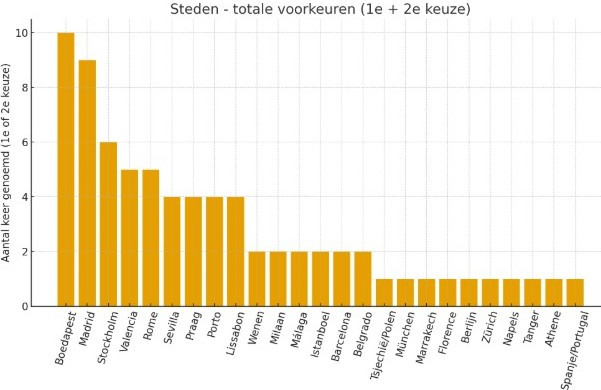
\includegraphics[width=\linewidth]{AllChoices}
	\label{fig:AllChoices}
	\caption{Alle antwoorden van de uitgezette pol.}
\end{figure}

\begin{figure}[h!]
	\centering
	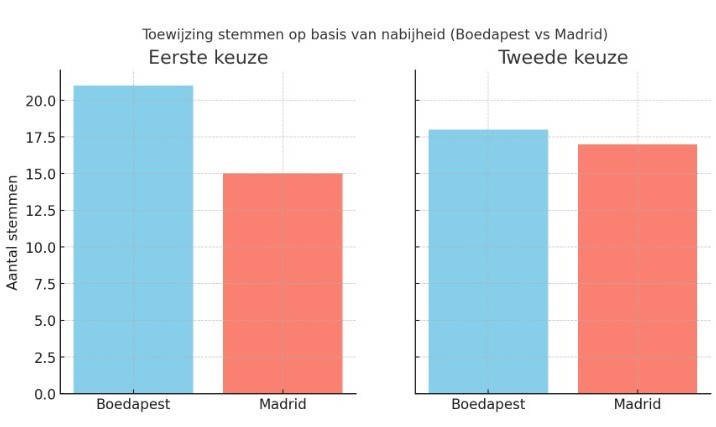
\includegraphics[width=\linewidth]{BudapestVSMadrid}
	\label{fig:MadridVsBoedapest}
	\caption{Boedapest vs Madrid.}
\end{figure}

Het programma van de reis is op dit moment nog in ontwikkeling. Aangezien dit projectplan een onderzoeks- en voorbereidingsdocument betreft, worden de definitieve invulling en details van het programma later vastgesteld. De opzet is om het programma samen met de studenten te bepalen door middel van aanvullende polls en door zelf onderzoek te doen naar interessante bedrijven en organisaties in de omgeving van Boedapest. Daarnaast zullen ook culturele en groepsversterkende activiteiten onderdeel uitmaken van het programma, zodat de reis zowel educatief als sociaal waardevol wordt.